\documentclass{standalone}
\usepackage{tikz}
\usetikzlibrary{patterns, positioning}

\begin{document}
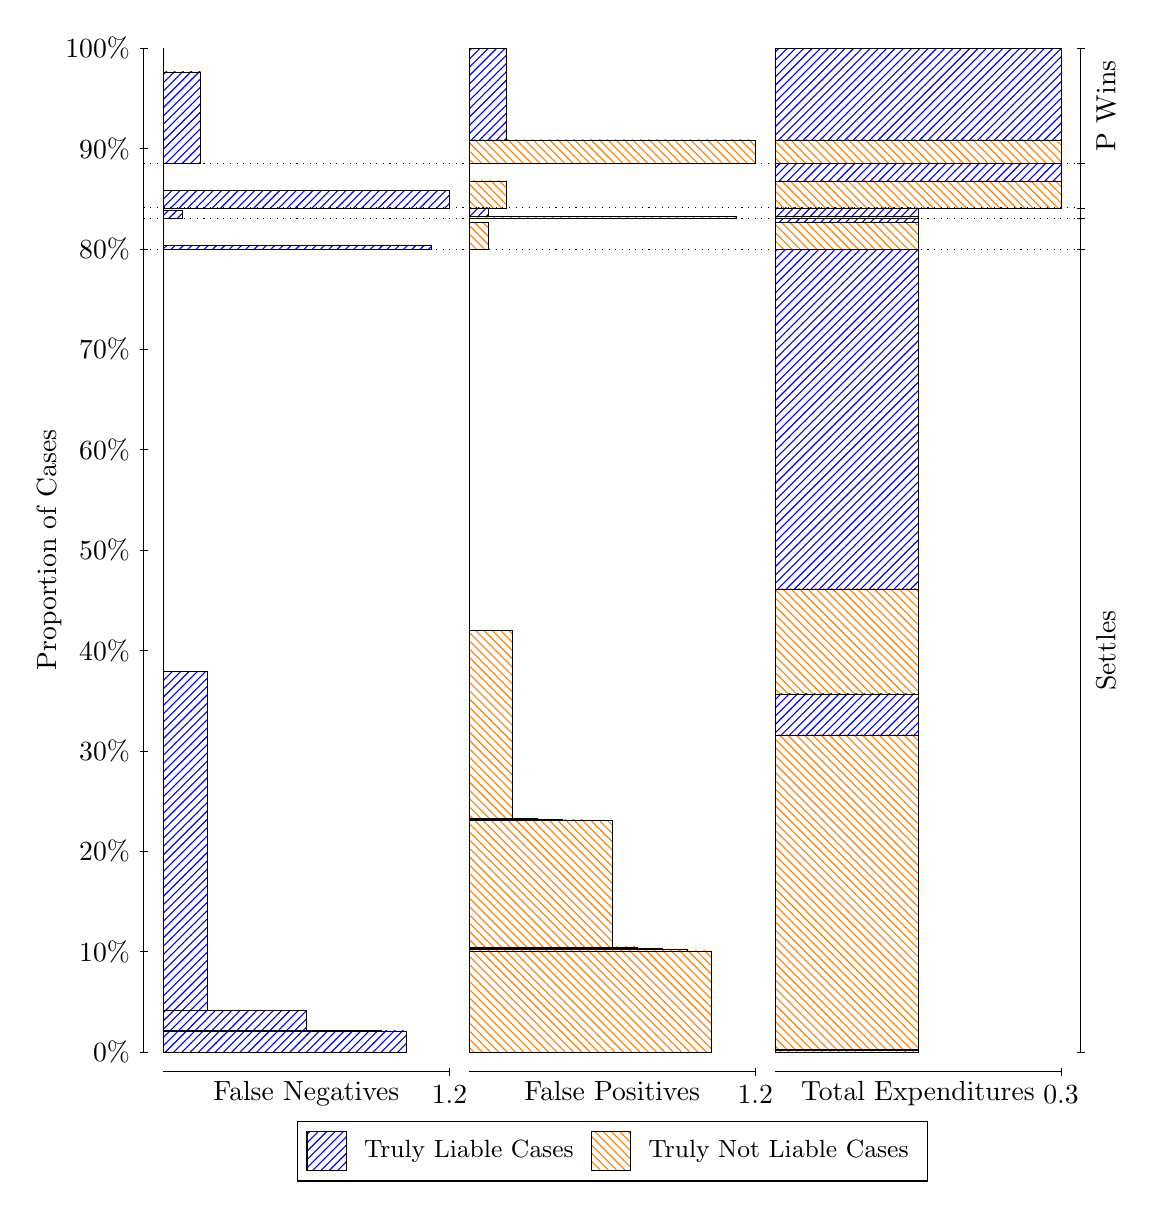
\begin{tikzpicture}
\draw[black, very thin] (1.5,1.75) -- (1.5,14.5);
\node[rotate=90, anchor=center] at (0.3, 8.125) {Proportion of Cases};
\draw[black, very thin] (1.45,1.75) -- (1.55,1.75);
\node[anchor=east] at (1.45, 1.75) {0\%};
\draw[black, very thin] (1.45,3.025) -- (1.55,3.025);
\node[anchor=east] at (1.45, 3.025) {10\%};
\draw[black, very thin] (1.45,4.3) -- (1.55,4.3);
\node[anchor=east] at (1.45, 4.3) {20\%};
\draw[black, very thin] (1.45,5.575) -- (1.55,5.575);
\node[anchor=east] at (1.45, 5.575) {30\%};
\draw[black, very thin] (1.45,6.85) -- (1.55,6.85);
\node[anchor=east] at (1.45, 6.85) {40\%};
\draw[black, very thin] (1.45,8.125) -- (1.55,8.125);
\node[anchor=east] at (1.45, 8.125) {50\%};
\draw[black, very thin] (1.45,9.4) -- (1.55,9.4);
\node[anchor=east] at (1.45, 9.4) {60\%};
\draw[black, very thin] (1.45,10.675) -- (1.55,10.675);
\node[anchor=east] at (1.45, 10.675) {70\%};
\draw[black, very thin] (1.45,11.95) -- (1.55,11.95);
\node[anchor=east] at (1.45, 11.95) {80\%};
\draw[black, very thin] (1.45,13.225) -- (1.55,13.225);
\node[anchor=east] at (1.45, 13.225) {90\%};
\draw[black, very thin] (1.45,14.5) -- (1.55,14.5);
\node[anchor=east] at (1.45, 14.5) {100\%};

\draw[black, very thin] (13.4,1.75) -- (13.4,14.5);
\draw[black, very thin] (13.35,1.75) -- (13.45,1.75);
\node[anchor=west] at (13.35, 1.75) {};
\draw[black, very thin] (13.35,11.939) -- (13.45,11.939);
\node[anchor=west] at (13.35, 11.939) {};
\draw[black, very thin] (13.35,12.338) -- (13.45,12.338);
\node[anchor=west] at (13.35, 12.338) {};
\draw[black, very thin] (13.35,12.471) -- (13.45,12.471);
\node[anchor=west] at (13.35, 12.471) {};
\draw[black, very thin] (13.35,13.031) -- (13.45,13.031);
\node[anchor=west] at (13.35, 13.031) {};
\draw[black, very thin] (13.35,14.5) -- (13.45,14.5);
\node[anchor=west] at (13.35, 14.5) {};

\draw[black, very thin, pattern color=blue, pattern=north east lines] (1.75,1.75) rectangle (4.8304,2.0183);
\draw[black, very thin, pattern color=blue, pattern=north east lines] (1.75,2.0183) rectangle (4.5145,2.0197);
\draw[black, very thin, pattern color=blue, pattern=north east lines] (1.75,2.0197) rectangle (4.1986,2.0212);
\draw[black, very thin, pattern color=blue, pattern=north east lines] (1.75,2.0212) rectangle (3.8826,2.0227);
\draw[black, very thin, pattern color=blue, pattern=north east lines] (1.75,2.0227) rectangle (3.5667,2.2744);
\draw[black, very thin, pattern color=blue, pattern=north east lines] (1.75,2.2744) rectangle (3.2507,2.2755);
\draw[black, very thin, pattern color=blue, pattern=north east lines] (1.75,2.2755) rectangle (2.9348,2.2767);
\draw[black, very thin, pattern color=blue, pattern=north east lines] (1.75,2.2767) rectangle (2.6188,2.2778);
\draw[black, very thin, pattern color=blue, pattern=north east lines] (1.75,2.2778) rectangle (2.3029,6.5828);
\draw[black, very thin, pattern color=orange, pattern=north west lines] (1.75,6.5828) rectangle (1.75,11.939);
\draw[black, very thin, pattern color=blue, pattern=north east lines] (1.75,11.939) rectangle (5.1464,11.993);
\draw[black, very thin, pattern color=orange, pattern=north west lines] (1.75,11.993) rectangle (1.75,12.338);
\draw[black, very thin, pattern color=blue, pattern=north east lines] (1.75,12.338) rectangle (1.987,12.442);
\draw[black, very thin, pattern color=orange, pattern=north west lines] (1.75,12.442) rectangle (1.75,12.471);
\draw[black, very thin, pattern color=blue, pattern=north east lines] (1.75,12.471) rectangle (5.3833,12.69);
\draw[black, very thin, pattern color=orange, pattern=north west lines] (1.75,12.69) rectangle (1.75,13.031);
\draw[black, very thin, pattern color=blue, pattern=north east lines] (1.75,13.031) rectangle (2.2239,14.196);
\draw[black, very thin, pattern color=orange, pattern=north west lines] (1.75,14.196) rectangle (1.75,14.5);
\draw[black, very thin, pattern color=orange, pattern=north west lines] (5.6333,1.75) rectangle (8.7138,3.0343);
\draw[black, very thin, pattern color=orange, pattern=north west lines] (5.6333,3.0343) rectangle (8.3978,3.051);
\draw[black, very thin, pattern color=orange, pattern=north west lines] (5.6333,3.051) rectangle (8.0819,3.0673);
\draw[black, very thin, pattern color=orange, pattern=north west lines] (5.6333,3.0673) rectangle (7.7659,3.0834);
\draw[black, very thin, pattern color=orange, pattern=north west lines] (5.6333,3.0834) rectangle (7.45,4.688);
\draw[black, very thin, pattern color=orange, pattern=north west lines] (5.6333,4.688) rectangle (7.1341,4.6881);
\draw[black, very thin, pattern color=orange, pattern=north west lines] (5.6333,4.6881) rectangle (7.1341,4.6971);
\draw[black, very thin, pattern color=orange, pattern=north west lines] (5.6333,4.6971) rectangle (6.8181,4.7061);
\draw[black, very thin, pattern color=orange, pattern=north west lines] (5.6333,4.7061) rectangle (6.5022,4.7149);
\draw[black, very thin, pattern color=orange, pattern=north west lines] (5.6333,4.7149) rectangle (6.1862,7.1065);
\draw[black, very thin, pattern color=blue, pattern=north east lines] (5.6333,7.1065) rectangle (5.6333,11.939);
\draw[black, very thin, pattern color=orange, pattern=north west lines] (5.6333,11.939) rectangle (5.8703,12.284);
\draw[black, very thin, pattern color=blue, pattern=north east lines] (5.6333,12.284) rectangle (5.6333,12.338);
\draw[black, very thin, pattern color=orange, pattern=north west lines] (5.6333,12.338) rectangle (9.0297,12.366);
\draw[black, very thin, pattern color=blue, pattern=north east lines] (5.6333,12.366) rectangle (5.8703,12.471);
\draw[black, very thin, pattern color=orange, pattern=north west lines] (5.6333,12.471) rectangle (6.1072,12.812);
\draw[black, very thin, pattern color=blue, pattern=north east lines] (5.6333,12.812) rectangle (5.6333,13.031);
\draw[black, very thin, pattern color=orange, pattern=north west lines] (5.6333,13.031) rectangle (9.2667,13.334);
\draw[black, very thin, pattern color=blue, pattern=north east lines] (5.6333,13.334) rectangle (6.1072,14.5);
\draw[black, very thin, pattern color=orange, pattern=north west lines] (9.5167,1.75) rectangle (11.333,1.7769);
\draw[black, very thin, pattern color=blue, pattern=north east lines] (9.5167,1.7769) rectangle (11.333,1.7813);
\draw[black, very thin, pattern color=orange, pattern=north west lines] (9.5167,1.7813) rectangle (11.333,5.7775);
\draw[black, very thin, pattern color=blue, pattern=north east lines] (9.5167,5.7775) rectangle (11.333,6.2975);
\draw[black, very thin, pattern color=orange, pattern=north west lines] (9.5167,6.2975) rectangle (11.333,7.6309);
\draw[black, very thin, pattern color=blue, pattern=north east lines] (9.5167,7.6309) rectangle (11.333,11.939);
\draw[black, very thin, pattern color=orange, pattern=north west lines] (9.5167,11.939) rectangle (11.333,12.284);
\draw[black, very thin, pattern color=blue, pattern=north east lines] (9.5167,12.284) rectangle (11.333,12.338);
\draw[black, very thin, pattern color=orange, pattern=north west lines] (9.5167,12.338) rectangle (11.333,12.366);
\draw[black, very thin, pattern color=blue, pattern=north east lines] (9.5167,12.366) rectangle (11.333,12.471);
\draw[black, very thin, pattern color=orange, pattern=north west lines] (9.5167,12.471) rectangle (13.15,12.812);
\draw[black, very thin, pattern color=blue, pattern=north east lines] (9.5167,12.812) rectangle (13.15,13.031);
\draw[black, very thin, pattern color=orange, pattern=north west lines] (9.5167,13.031) rectangle (13.15,13.334);
\draw[black, very thin, pattern color=blue, pattern=north east lines] (9.5167,13.334) rectangle (13.15,14.5);
\draw[black, dotted] (1.5,11.939) -- (13.4,11.939);
\draw[black, dotted] (1.5,12.338) -- (13.4,12.338);
\draw[black, dotted] (1.5,12.471) -- (13.4,12.471);
\draw[black, dotted] (1.5,13.031) -- (13.4,13.031);
\draw[black, very thin] (1.75,1.5) -- (5.3833,1.5);
\node[anchor=north] at (3.5667, 1.5) {False Negatives};
\draw[black, very thin] (5.3833,1.45) -- (5.3833,1.55);
\node[anchor=north] at (5.3833, 1.45) {1.2};

\draw[black, very thin] (5.6333,1.5) -- (9.2667,1.5);
\node[anchor=north] at (7.45, 1.5) {False Positives};
\draw[black, very thin] (9.2667,1.45) -- (9.2667,1.55);
\node[anchor=north] at (9.2667, 1.45) {1.2};

\draw[black, very thin] (9.5167,1.5) -- (13.15,1.5);
\node[anchor=north] at (11.333, 1.5) {Total Expenditures};
\draw[black, very thin] (13.15,1.45) -- (13.15,1.55);
\node[anchor=north] at (13.15, 1.45) {0.3};

\node[black, centered, rotate=90] at (13.72, 6.8447) {Settles};



\node[black, centered, rotate=90] at (13.72, 13.765) {P Wins};

\draw (7.449999999999999,1.5) node[draw=none] (baseCoordinate) {};
\begin{scope}[align=center]
        \matrix[scale=0.5, draw=black, below=0.5cm of baseCoordinate, nodes={draw}, column sep=0.1cm]{
            \node[rectangle, draw, minimum width=0.5cm, minimum height=0.5cm, pattern=north east lines, pattern color=blue] {}; &
            \node[draw=none, font=\small] (B) {Truly Liable Cases}; &
            \node[rectangle, draw, minimum width=0.5cm, minimum height=0.5cm, pattern=north west lines, pattern color=orange] {}; &
            \node[draw=none, font=\small] (B) {Truly Not Liable Cases}; \\
            };
\end{scope}

\end{tikzpicture}
\end{document}